% ----------------------------------------------------------------------------
%                           FUNDAMENTAÇÃO TEÓRICA
% ----------------------------------------------------------------------------

\chapter{FUNDAMENTAÇÃO TEÓRICA}
\label{chap:fundamentacao}

Para fundamentar o desenvolvimento da solução tecnológica proposta neste trabalho, torna-se necessário analisar sistemas correlatos já existentes, com o objetivo de compreender como diferentes plataformas abordam aspectos relacionados ao manejo comportamental, à comunicação escolar e à organização de rotinas voltadas ao público neurodivergente. Essa análise permite identificar funcionalidades relevantes, estratégias de interação e, sobretudo, limitações e lacunas ainda presentes nas soluções disponíveis, justificando a proposição de um novo sistema.

Nesse contexto, são investigados cinco sistemas com diferentes finalidades e abordagens: o DBT Coach, voltado ao acompanhamento clínico e emocional; o ClassDojo, direcionado à gamificação da comunicação entre escola e família; o Pictalk Buddy e o Minha Rotina Especial, focados na organização visual de rotinas e no suporte à previsibilidade das atividades diárias; e a Sequência Mágica, ferramenta educacional voltada ao desenvolvimento da organização lógica e sequencial na educação infantil.

A análise comparativa considera aspectos como objetivo da plataforma, público-alvo, funcionalidades oferecidas, recursos de acessibilidade, estratégias de interação e usabilidade estrutural. A partir dessa investigação, busca-se compreender de que maneira as soluções existentes podem contribuir para a construção de uma proposta mais integrada, acessível e adequada às necessidades de crianças neurodivergentes, seus responsáveis e profissionais da educação.

\section{Sistemas Similares}

A fim de mapear o panorama tecnológico atual e identificar as lacunas existentes no mercado educacional e de saúde, esta seção apresenta uma análise de sistemas similares voltados ao suporte comportamental e à regulação emocional. A partir dessa investigação, torna-se possível contrastar as soluções já consolidadas com a proposta inovadora delineada neste trabalho.

\vspace{0.3cm}
\subsection{DBT Coach}

O DBT Coach \textit{(Dialectical Behavior Therapy)} é um aplicativo disponível para dispositivos móveis \textit{(Google Play e App Store)} desenvolvido para auxiliar no ensino de habilidades de regulação emocional, conforme informações do seu site oficial \cite{swasth2026}. O software fundamenta-se nos princípios da Terapia Comportamental Dialética e tem como propósito central oferecer suporte clínico para o manejo de crises. Seu público-alvo é composto por pacientes em acompanhamento psicológico e terapeutas que buscam monitorar a evolução do tratamento de forma remota.

O software permite o registro estruturado de estados emocionais e comportamentos por meio da análise funcional (Antecedente, Comportamento e Consequência). Entre suas principais funcionalidades, o aplicativo oferece sugestões de intervenção em tempo real e módulos de treinamento de habilidades. O sistema gera alertas e lembretes baseados no nível de estresse reportado pelo usuário, funcionando como uma ferramenta de suporte imediato para momentos de desregulação.

Em relação à usabilidade, o sistema apresenta uma interface densa e técnica, voltada ao ambiente de saúde mental. Conforme ilustrado na Figura 2.1, a tela principal utiliza um esquema de cores escuras e organiza as funções em um grid de botões para registros rápidos, identificados por ícones para Emoção, Impulso, Comportamento e Sono. A tela de registro clínico exibe uma lista detalhada de comportamentos-alvo, como autolesão e agressão, permitindo que o usuário selecione a intensidade e a frequência de cada ocorrência por meio de seletores táteis.
\begin{figure}[H] 
    \centering
    \caption{Telas principais do aplicativo DBT Coach} % <-- Legenda ÚNICA no topo
    \label{fig:telas_dbt}
    \vspace{0.3cm}
    
    % --- Imagem A ---
    \begin{minipage}[b]{0.46\textwidth}
        \centering
        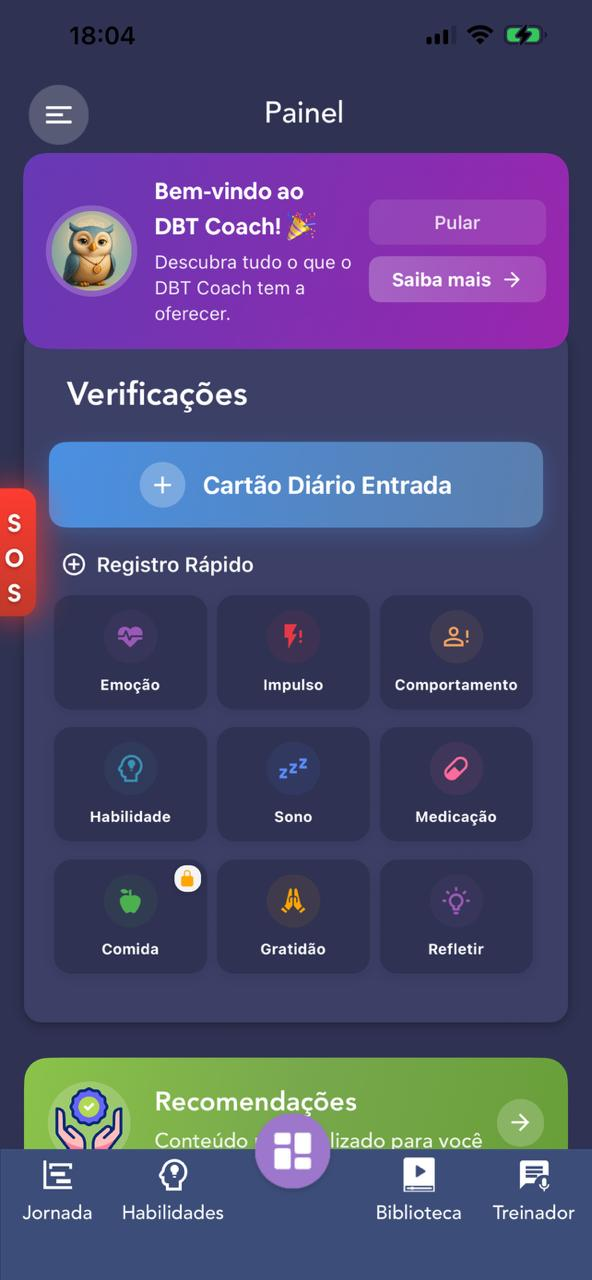
\includegraphics[height=9cm, keepaspectratio]{dados/figuras/telaDBTCoach_1} 
        \centerline{\small (a) Interface de registros} % <-- Subtítulo A
    \end{minipage}\hfill
    % --- Imagem B ---
    \begin{minipage}[b]{0.46\textwidth}
        \centering
        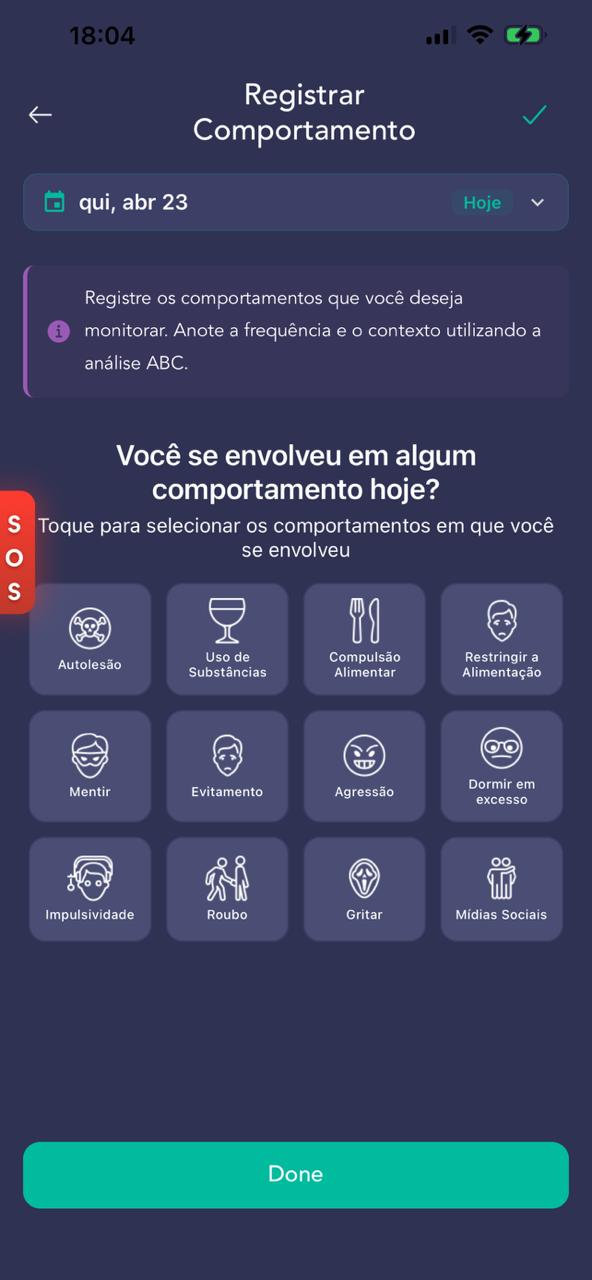
\includegraphics[height=9cm, keepaspectratio]{dados/figuras/telaDBTCoach_2}
        \centerline{\small (b) Painel clínico} % <-- Subtítulo B
    \end{minipage}
    
   \vspace{0.3cm}
    \begin{flushleft} % <-- Inicia o alinhamento à esquerda
        \footnotesize Fonte: DBT Coach (2026) % <-- Sem o \legend, apenas o texto!
    \end{flushleft}   
\end{figure}

\vspace{0.3cm}
\subsection{ClassDojo}

O ClassDojo é uma plataforma de gestão escolar e comunicação disponível via web e em aplicativos móveis, amplamente utilizada para conectar a escola à família \cite{classdojo2026}. O software tem como propósito central a gamificação do comportamento em sala de aula e a criação de uma comunidade escolar integrada. Seu público-alvo principal são professores da educação básica, alunos e seus respectivos responsáveis.

O software permite a criação de turmas digitais onde cada aluno é representado por um avatar personalizável. As principais funcionalidades incluem o compartilhamento de fotos e vídeos das atividades e um sistema de atribuição de pontos. Os professores podem configurar competências positivas ou pontos a melhorar, emitindo relatórios automáticos sobre o engajamento dos estudantes. O aplicativo ainda permite a troca de mensagens diretas e privadas entre a escola e os pais.

A interface do aplicativo aposta em um design lúdico e colorido para atrair o público infantil. Conforme ilustrado na Figura 2.2, a tela de gestão da turma apresenta avatares em formato de monstrinhos que mudam conforme a pontuação recebida. Ao selecionar um aluno, o sistema abre um menu flutuante com ícones verdes para reforços positivos (como "Trabalho duro") e ícones vermelhos com sinal de menos (-1) para comportamentos que precisam de ajuste (como "Falta de foco"), oferecendo um feedback visual imediato sobre a conduta do estudante.
\begin{figure}[H] 
    \centering
    \caption{Telas principais do aplicativo ClassDojo} % <-- Legenda ÚNICA no topo
    \label{fig:telas_dbt}
    \vspace{0.3cm}
    
    % --- Imagem A ---
    \begin{minipage}[b]{0.46\textwidth}
        \centering
        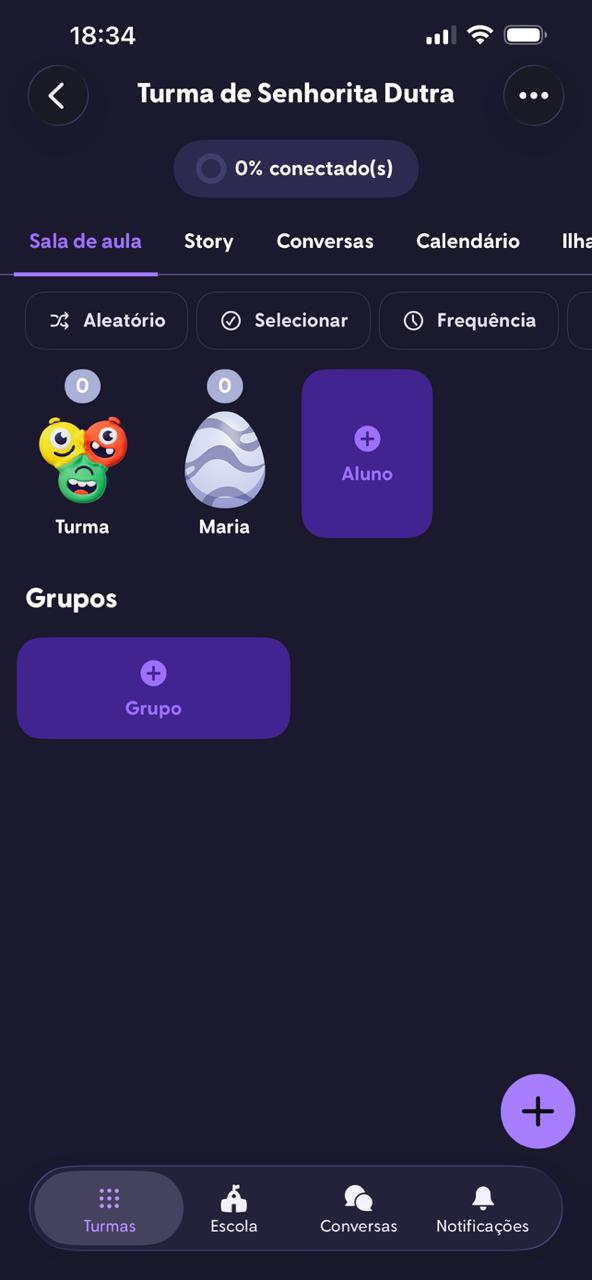
\includegraphics[height=9cm, keepaspectratio]{dados/figuras/telaClassDojo_1} 
        \centerline{\small (a) Visão geral da turma} % <-- Subtítulo A
    \end{minipage}\hfill
    % --- Imagem B ---
    \begin{minipage}[b]{0.46\textwidth}
        \centering
        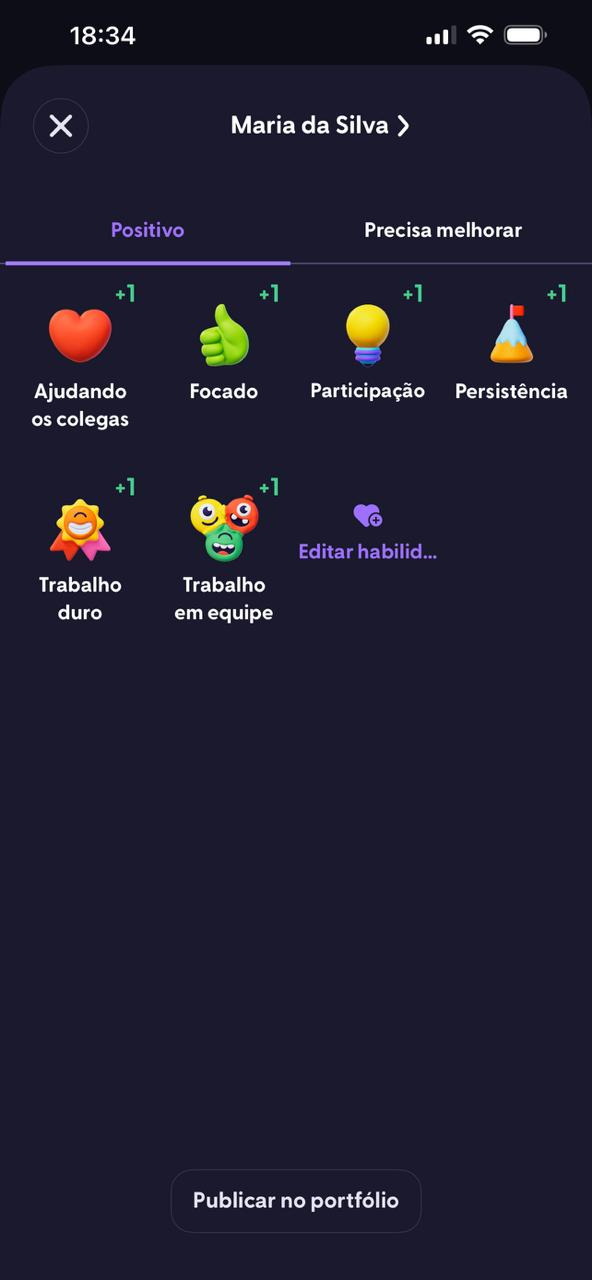
\includegraphics[height=9cm, keepaspectratio]{dados/figuras/telaClassDojo_2}
        \centerline{\small (b) Interface de pontuações} % <-- Subtítulo B
    \end{minipage}
    
    \vspace{0.3cm}
    \begin{flushleft} % <-- Inicia o alinhamento à esquerda
    \footnotesize{Fonte: ClassDojo (2026)} % <-- Fonte ÚNICA no final
 \end{flushleft}   
\end{figure}

\vspace{0.2cm}

Contudo, o sistema apresenta falhas metodológicas quando aplicado ao público com TDAH e TOD. O modelo de gamificação baseada em punição pública (perda de pontos visível) pode gerar ansiedade e reforçar o comportamento opositor. Adicionalmente, as avaliações de usuários indicam que o software falha ao não permitir o registro detalhado e privado de ocorrências comportamentais complexas, transformando a comunicação em uma linha do tempo genérica que não orienta os pais sobre como intervir tecnicamente em casa. 

\vspace{0.3cm}
\subsection{Pictalk Buddy}
 
 O Pictalk Buddy é um aplicativo de tecnologia assistiva disponível para smartphones, desenvolvido por uma organização focada em acessibilidade cognitiva \cite{pictalk2026}. O software permite a criação de agendas visuais para auxiliar pessoas com dificuldades na função executiva. Seu público-alvo compreende crianças e adultos com TEA, TDAH e outras condições que se beneficiam da previsibilidade das tarefas diárias.

O software permite a criação passo a passo das rotinas por meio de pictogramas e recursos de voz. As principais funcionalidades envolvem a organização sequencial de atividades, onde o aplicativo gera alertas sonoros que lembram o usuário sobre cada etapa a ser realizada. O sistema também oferece suporte para comunicação alternativa, permitindo que o usuário expresse necessidades básicas através de imagens caso encontre dificuldades na fala verbal.

A usabilidade do Pictalk Buddy é pautada na clareza visual e no minimalismo para evitar a sobrecarga sensorial. Conforme ilustrado na Figura 2.3, a interface é composta por grandes cartões quadrados que contêm ilustrações simples de tarefas cotidianas, como "Escovar os dentes" ou "Lanche". Abaixo de cada imagem, há uma legenda em texto e um botão de áudio; ao ser tocado, o aplicativo narra a instrução em voz alta, permitindo que o usuário avance na rotina de forma autônoma e acompanhe visualmente o progresso do seu dia.
\begin{figure}[H] 
    \centering
    \caption{Telas principais do aplicativo PicTalk} % <-- Legenda ÚNICA no topo
    \label{fig:telas_dbt}
    \vspace{0.3cm}
    
    % --- Imagem A ---
    \begin{minipage}[b]{0.46\textwidth}
        \centering
        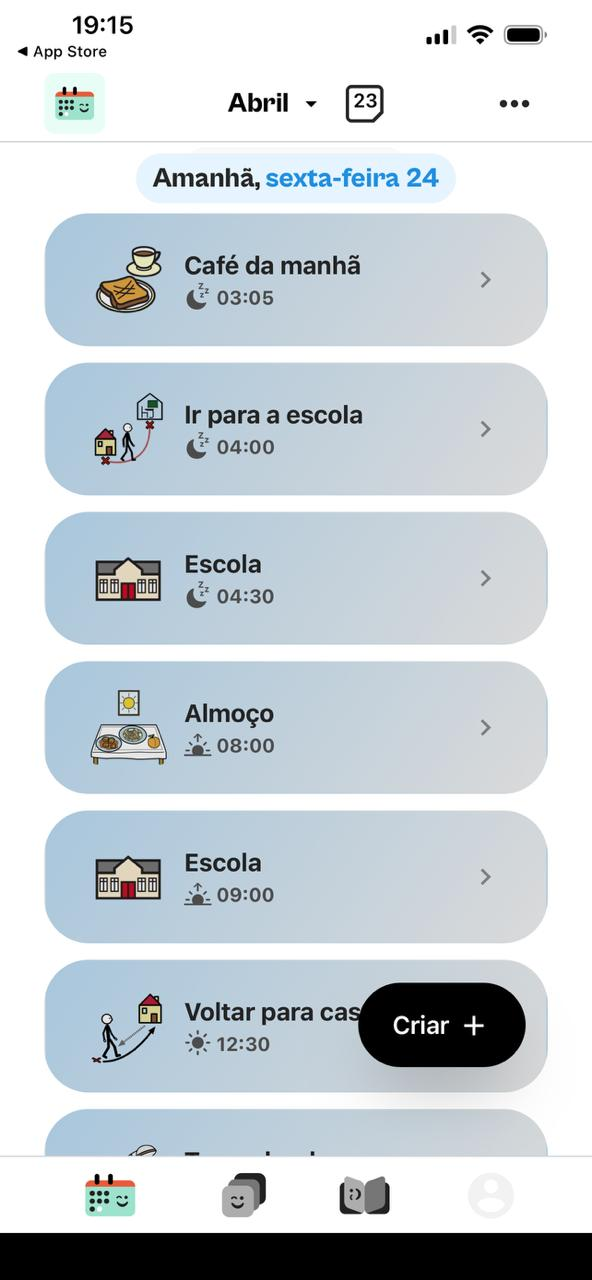
\includegraphics[height=9cm, keepaspectratio]{dados/figuras/telaPicTalk_1} 
        \centerline{\small (a) Agenda visual no aplicativo} % <-- Subtítulo A
    \end{minipage}\hfill
    % --- Imagem B ---
    \begin{minipage}[b]{0.46\textwidth}
        \centering
        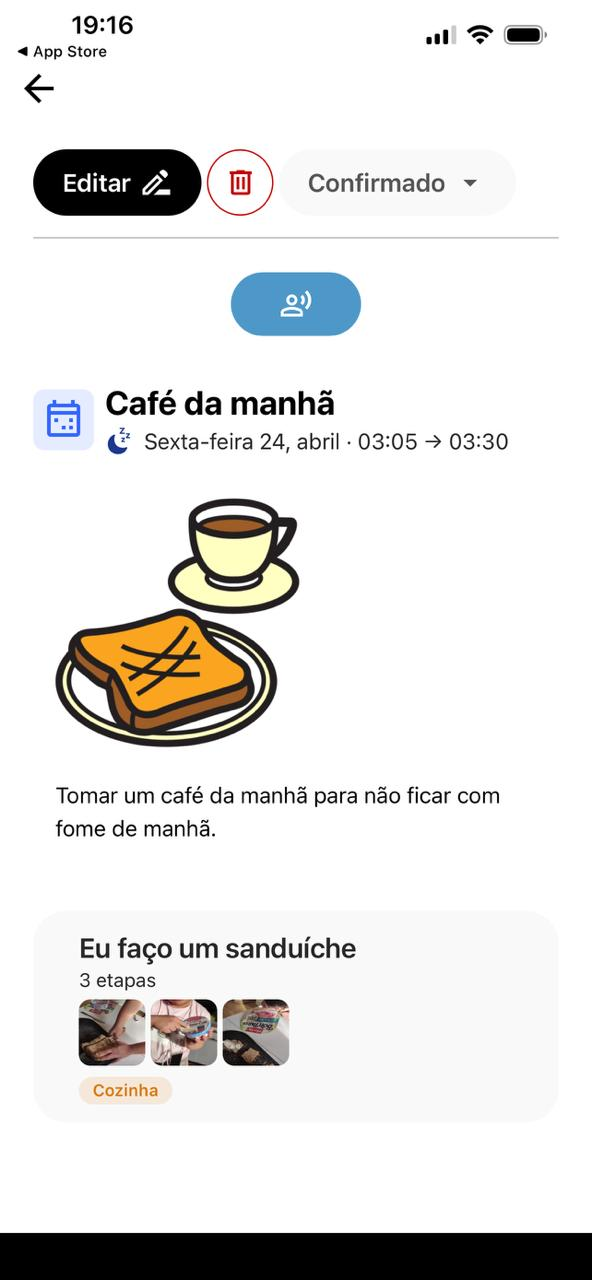
\includegraphics[height=9cm, keepaspectratio]{dados/figuras/telaPicTalk_2}
        \centerline{\small (b) Organização de agenda de café da manhã} % <-- Subtítulo B
    \end{minipage}
    
  \vspace{0.3cm}
    \begin{flushleft} % <-- Inicia o alinhamento à esquerda
   \footnotesize{Fonte: PicTalk (2026)} % <-- Fonte ÚNICA no final
 \end{flushleft}   
\end{figure}

\vspace{0.2cm}
Apesar de ser eficaz na promoção da autonomia individual, a ferramenta não supre as necessidades de uma gestão escolar compartilhada. Por ser um aplicativo pago e focado no uso pessoal da criança, ele não oferece recursos para que o professor registre comportamentos desafiadores ou alinhe estratégias táticas com os pais. O software atua na prevenção por meio da rotina, mas falha em prover um canal de comunicação e suporte para o manejo comportamental reativo necessário no contexto do TDAH e do TOD.

\vspace{0.3cm}
\subsection{Sequência Mágica}

O sistema web "Sequência Mágica", desenvolvido como pesquisa acadêmica no Instituto Federal de Brasília \cite{santos2025}, é uma plataforma interativa voltada para a organização de rotinas. O propósito principal da ferramenta é auxiliar no desenvolvimento da autonomia e do raciocínio lógico por meio da estruturação de atividades cotidianas. Seu público-alvo direto compreende crianças de 2 a 4 anos diagnosticadas com Transtorno do Espectro Autista (TEA), bem como educadores da primeira infância e pais que auxiliam na mediação dessas atividades.

As principais funcionalidades do sistema baseiam-se na criação interativa de sequências visuais. A plataforma permite que o usuário selecione blocos representativos de ações do dia a dia (como "acordar", "tomar banho" e "escovar os dentes") e os posicione na ordem correta utilizando o recurso de arrastar e soltar (drag and drop). Além disso, o software possui recursos para salvar a rotina montada no armazenamento local do navegador (localStorage), permitindo a visualização, restauração ou exclusão de sequências previamente configuradas e associadas à data atual.

A Figura 2.4 apresenta as telas principais do protótipo do sistema Sequência Mágica. Em relação à usabilidade, o aplicativo adota uma interface voltada para a acessibilidade cognitiva do público infantil, priorizando a clareza visual e a simplicidade de navegação. Como pode ser observado na tela de início (a), há o uso de personagens lúdicos e cores suaves que geram empatia imediata. Já na tela de montagem da sequência (b), a estruturação utiliza uma barra lateral com blocos de rotina diária (como acordar e tomar banho), representados por pictogramas coloridos e legendas simples. Essa disposição limpa e interativa no painel principal permite que a criança acompanhe e estruture o seu próprio dia de forma intuitiva, promovendo a previsibilidade e evitando a sobrecarga sensorial.
\begin{figure}[H] 
    \centering
    \caption{Telas principais do protótipo de Sequência Mágica} % <-- Legenda ÚNICA no topo
    \label{fig:telas_dbt}
    \vspace{0.3cm}
    
    % --- Imagem A ---
    \begin{minipage}[b]{0.46\textwidth}
        \centering
        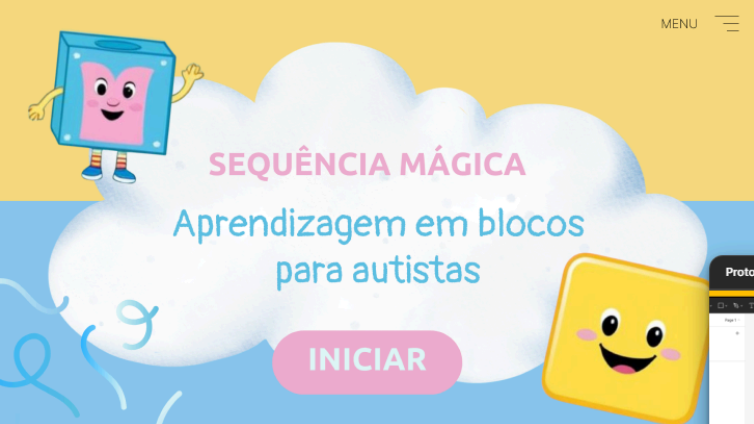
\includegraphics[height=9cm, keepaspectratio]{dados/figuras/telaSequenciaMagica_1} 
        \centerline{\small (a) Tela de início} % <-- Subtítulo A
    \end{minipage}\hfill
    % --- Imagem B ---
    \begin{minipage}[b]{0.46\textwidth}
        \centering
        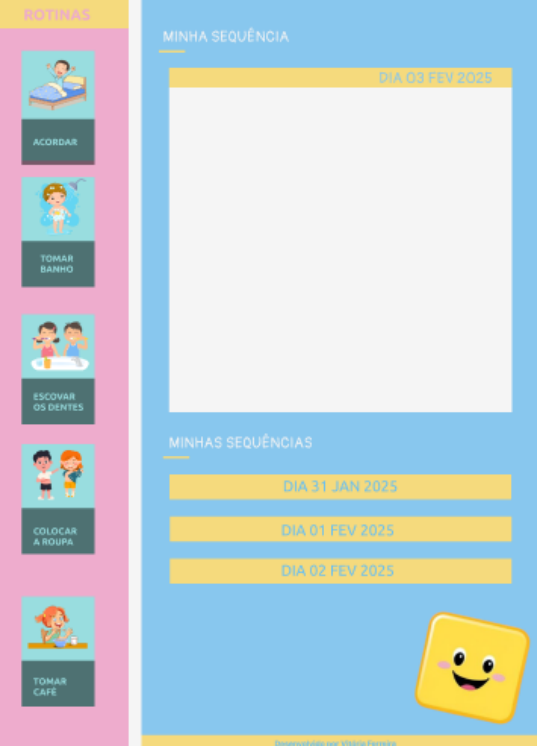
\includegraphics[height=9cm, keepaspectratio]{dados/figuras/telaSequenciaMagica_2}
        \centerline{\small (b)  Tela de montagem da sequência dos cards} % <-- Subtítulo B
    \end{minipage}
    
   \vspace{0.3cm}
    \begin{flushleft} % <-- Inicia o alinhamento à esquerda
   \footnotesize{Fonte: Silva (2025, p. 30, 31).} % <-- Fonte ÚNICA no final
 \end{flushleft}   
\end{figure}

\vspace{0.2cm}
Apesar de ser uma iniciativa acadêmica de excelência para a educação infantil, a plataforma apresenta limitações metodológicas e técnicas frente aos objetivos deste projeto. O primeiro obstáculo é estrutural: por utilizar o armazenamento local (localStorage) e não possuir sistema de autenticação ou banco de dados em nuvem, o aplicativo restringe os dados a um único dispositivo, impedindo o compartilhamento de informações integradas entre a escola e a família. Ademais, por focar estritamente na organização preventiva de rotinas para crianças de 2 a 4 anos, a ferramenta não contempla um módulo de comunicação escolar, registro de ocorrências ou suporte tático para o manejo reativo de crises associadas ao TDAH e ao TOD no ambiente educacional.
\vspace{0.3cm}

\section{Análise Comparativa}

Após a análise individual das ferramentas, o Quadro \ref{quadro:comparativo_sistemas} apresenta uma síntese comparativa. Fica evidente que, embora existam soluções robustas para a comunicação alternativa (PicTalk), gamificação (ClassDojo) ou rotinas diárias (Sequência Mágica), há uma lacuna no que diz respeito a um sistema escolar que integre o registro de ocorrências à oferta ativa de estratégias de manejo para professores de alunos com TDAH e TOD, necessidade esta que a solução proposta visa suprir.

\begin{table}[H]
    \centering
    \caption{Comparativo entre os sistemas similares e a solução proposta}
    \label{quadro:comparativo_sistemas}
    \renewcommand{\arraystretch}{1.4} 
    \setlength{\tabcolsep}{3pt}
    \small 

    \begin{tabular}{|p{2.4cm}|p{3.8cm}|p{2.5cm}|p{2.4cm}|p{2.0cm}|p{1.8cm}|}
        \hline
        \textbf{Sistema} & \textbf{Foco Principal} & \textbf{Público-Alvo} & \textbf{Comunicação \newline Escola-Família} & \textbf{Sugestões \newline de Manejo} & \textbf{Plataforma} \\ \hline
        
        \textbf{DBT Coach} & Regulação emocional e habilidades de enfrentamento clínico. & Pacientes e terapeutas & Não & Sim (Clínico) & App Mobile \\ \hline
        
        \textbf{ClassDojo} & Gestão de sala de aula, engajamento e gamificação de comportamento. & Professores, pais e alunos & Sim & Não & Web e Mobile \\ \hline
        
        \textbf{PicTalk} & Comunicação Alternativa e Aumentativa (CAA) com pictogramas. & Crianças, pais e terapeutas & Não & Não & App Mobile \\ \hline
        
        \textbf{Sequência Mágica} & Organização de rotinas diárias e acessibilidade cognitiva. & Crianças e pais & Não & Não & App Mobile \\ \hline
        
        \textbf{Sistema Proposto} & Registro comportamental contínuo e suporte estratégico pedagógico. & Professores e pais \newline (Foco em TDAH/TOD) & Sim & Sim & Web Resp. \\ \hline
    \end{tabular}
    
    \vspace{0.2cm}
    \legend{Fonte: Elaborado pelo autor (2026)}
\end{table}

\vspace{0.3cm}
\section{Considerações do Capítulo}

Este capítulo apresentou os principais sistemas e conceitos que fundamentam a pesquisa, abordando ferramentas voltadas ao manejo do Transtorno de Déficit de Atenção com Hiperatividade (TDAH) e do Transtorno Opositor Desafiador (TOD), bem como plataformas de comunicação escolar e tecnologias de regulação emocional. A análise comparativa desses recursos forneceu a base necessária para a compreensão das necessidades da rede de apoio (escola e família) e evidenciou a lacuna tecnológica existente no mercado, justificando e sustentando o desenvolvimento da proposta apresentada nos capítulos seguintes.